\documentclass[aspectratio=169]{beamer}

% ============================================
% PACOTES ADICIONAIS
% ============================================
\usepackage[utf8]{inputenc}
\usepackage[T1]{fontenc}
\usepackage{amsmath}
\usepackage{amsfonts}
\usepackage{amssymb}
\usepackage{graphicx}
\usepackage{cite}
\usepackage{url}
\usepackage{hyperref}
\usepackage{ifthen}
\usepackage{bm}
\usepackage{array}
\usepackage{tikz}
\usepackage{pgfplots}
\pgfplotsset{compat=1.18}
\usetikzlibrary{shapes.geometric, arrows.meta, positioning, decorations.pathreplacing,
                calc, fit, backgrounds, shadows}

% ============================================
% VARIAVEIS DE CONFIGURACAO
% ============================================
\newcommand{\autorNome}{Prof. Daniel Costa Araujo}
\newcommand{\autorEmail}{daniel.araujo@unb.br}
\newcommand{\tituloApresentacao}{Principios de Comunicacao para Engenharia}
\newcommand{\subtituloApresentacao}{Apresentacao da Disciplina}
\newcommand{\idioma}{pt}
\newcommand{\universidadePT}{Universidade de Brasilia}
\newcommand{\departamentoPT}{Faculdade de Ciencias e Tecnologia em Engenharias}
\newcommand{\laboratorioPT}{Laboratorio de Telecomunicacoes}
\newcommand{\universidadeEN}{University of Brasilia}
\newcommand{\departamentoEN}{Faculty of Sciences and Technology in Engineering}
\newcommand{\laboratorioEN}{Telecommunications Laboratory}
\newcommand{\dataApresentacao}{17 de Março de 2026}

\newcommand{\institutoFinal}{%
    \ifthenelse{\equal{\idioma}{pt}}{\universidadePT \\ \laboratorioPT}%
                                    {\universidadeEN \\ \laboratorioEN}%
}
\newcommand{\universidadeFinal}{%
    \ifthenelse{\equal{\idioma}{pt}}{\universidadePT}{\universidadeEN}%
}
\newcommand{\laboratorioFinal}{%
    \ifthenelse{\equal{\idioma}{pt}}{\laboratorioPT}{\laboratorioEN}%
}

% ============================================
% Backup color definition (template redefines)
\definecolor{unbprimary}{RGB}{0,59,92}
\colorlet{cOrange}{orange!80!black}
\colorlet{cBlue}{blue!70!black}
\colorlet{cTeal}{teal!70!black}
\colorlet{cRed}{red!60!black}
\colorlet{cPurple}{purple!70!black}
\colorlet{cGreen}{green!50!black}
% CARREGAR TEMPLATE UnB/LabTelecom
% ============================================
% Template Beamer para UnB/LabTelecom
% Cores da UnB
\definecolor{unbprimary}{RGB}{0,59,92}      % #003B5C
\definecolor{unbsecondary}{RGB}{0,102,51}   % #006633
\definecolor{unbaccent}{RGB}{242,169,0}      % #F2A900


% Configuração do tema
\usetheme{Madrid}
\usecolortheme{default}

% Aplicar cores UnB
\setbeamercolor{structure}{fg=unbprimary}
\setbeamercolor{title}{fg=white}
\setbeamercolor{frametitle}{fg=white}
\setbeamercolor{section in toc}{fg=unbprimary}
\setbeamercolor{subsection in toc}{fg=unbsecondary}

% Configurações de fonte
\setbeamerfont{title}{size=\huge,series=\bfseries}
\setbeamerfont{frametitle}{size=\Large,series=\bfseries}



% Cabeçalho com logos
\setbeamertemplate{headline}{
  \begin{beamercolorbox}[wd=\paperwidth,ht=1.2cm]{headline}
    \hspace{0.5cm}%
    \raisebox{0.2cm}{
\includegraphics[height=0.8cm]{../../figures_global/unb.png}}%
    \hfill%
    \raisebox{0.35cm}{\textcolor{unbprimary}{\textbf{\universidadeFinal}}}%
    \hfill%
    \raisebox{0.2cm}{
\includegraphics[height=0.8cm]{../../figures_global/labtelecom.png}}%
    \hspace{0.5cm}%
  \end{beamercolorbox}
}

% Rodapé
\setbeamertemplate{footline}{
  \begin{beamercolorbox}[wd=\paperwidth,ht=0.5cm]{footline}
    \hspace{1cm}
    \textcolor{unbprimary}{\insertshorttitle}
    \hfill
    \textcolor{unbprimary}{\insertframenumber/\inserttotalframenumber}
    \hspace{1cm}
  \end{beamercolorbox}
}

% Remover símbolos de navegação e mini frames (evita conflito com TikZ)
\setbeamertemplate{navigation symbols}{}
\setbeamertemplate{mini frames}{}
\setbeamertemplate{mini frame in current subsection}{}
\setbeamertemplate{mini frame in other section}[default]

% ============================================
% APLICAR CONFIGURACOES
% ============================================
\title{\tituloApresentacao}
\subtitle{\subtituloApresentacao}
\author{\autorNome}
\institute{\institutoFinal}
\date{\dataApresentacao}

% Comandos uteis
\newcommand{\vect}[1]{\mathbf{#1}}
\newcommand{\figFull}{0.85\textwidth}
\newcommand{\figHalf}{0.65\textwidth}
\newcommand{\figHalfV}{0.48\textwidth}
\newcommand{\figw}{\figFull}

% ============================================
\begin{document}

% --- TITULO ---
\begin{frame}
\titlepage
\end{frame}

% --- SUMARIO ---
\begin{frame}{Sum\'{a}rio (1/2)}
\tableofcontents[hideallsubsections, sections={1-3}]
\end{frame}

\begin{frame}{Sum\'{a}rio (2/2)}
\tableofcontents[hideallsubsections, sections={4-6}]
\end{frame}

% %%%%%%%%%%%%%%%%%%%%%%%%%%%%%%%%%%%%%%%%%%%%
\section{Por que Comunicac\~{o}es?}
% %%%%%%%%%%%%%%%%%%%%%%%%%%%%%%%%%%%%%%%%%%%%

{
\setbeamercolor{background canvas}{bg=unbprimary}
\setbeamercolor{normal text}{fg=white}
\usebeamercolor[fg]{normal text}
\begin{frame}[plain,c]
\begin{center}
{\Huge\textbf{Por que Comunicac\~{o}es?}}\\[0.8cm]
{\LARGE Tudo ao nosso redor \'{e} comunicac\~{a}o}\\[0.5cm]
{\large Sinais, espectro, modulac\~{a}o --- a linguagem do mundo moderno}
\end{center}
\end{frame}
}

\begin{frame}[t]{Estamos rodeados por comunicac\~{o}es}
\begin{columns}
\begin{column}{0.52\textwidth}
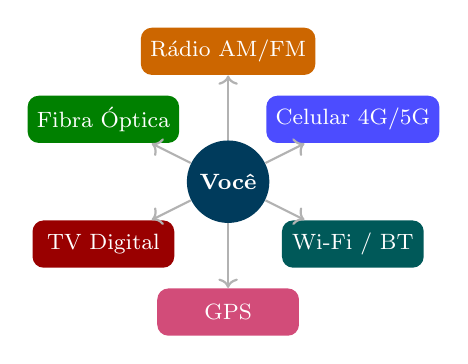
\begin{tikzpicture}[scale=0.72]
  \node[circle, fill=unbprimary, text=white, minimum size=1.0cm,
        font=\footnotesize\bfseries] (you) at (0,0) {Voc\^{e}};
  \node[rounded corners, fill=orange!80!black, text=white, minimum width=1.8cm,
        minimum height=0.6cm, align=center, font=\footnotesize]
    (radio) at (0, 2.3) {R\'{a}dio AM/FM};
  \node[rounded corners, fill=blue!70, text=white, minimum width=1.8cm,
        minimum height=0.6cm, align=center, font=\footnotesize]
    (cell) at (2.2, 1.1) {Celular 4G/5G};
  \node[rounded corners, fill=teal!70!black, text=white, minimum width=1.8cm,
        minimum height=0.6cm, align=center, font=\footnotesize]
    (wifi) at (2.2,-1.1) {Wi-Fi / BT};
  \node[rounded corners, fill=purple!70, text=white, minimum width=1.8cm,
        minimum height=0.6cm, align=center, font=\footnotesize]
    (gps) at (0,-2.3) {GPS};
  \node[rounded corners, fill=red!60!black, text=white, minimum width=1.8cm,
        minimum height=0.6cm, align=center, font=\footnotesize]
    (tv) at (-2.2,-1.1) {TV Digital};
  \node[rounded corners, fill=green!50!black, text=white, minimum width=1.8cm,
        minimum height=0.6cm, align=center, font=\footnotesize]
    (fiber) at (-2.2, 1.1) {Fibra \'{O}ptica};
  \foreach \n in {radio, cell, wifi, gps, tv, fiber}
    \draw[->, thick, gray!60] (you) -- (\n);
\end{tikzpicture}
\end{column}
\begin{column}{0.45\textwidth}
  \small\textbf{Exemplos do dia a dia:}
  \begin{itemize}\setlength{\itemsep}{1pt}
    \item \textbf{R\'{a}dio AM/FM} --- mod. amplitude/frequ\^{e}ncia
    \item \textbf{Celular 4G/5G} --- OFDM, MIMO
    \item \textbf{Wi-Fi} --- IEEE 802.11, m\'{u}lt. portadoras
    \item \textbf{GPS} --- CDMA, c\'{o}digo pseudo-aleat\'{o}rio
    \item \textbf{TV Digital} --- ISDB-T, FEC
    \item \textbf{Fibra \'{O}ptica} --- WDM
  \end{itemize}
  \vspace{0.15cm}
  \textbf{O que \'{e} comum a todos?}\\
  \alert{Sinais, espectro e modulac\~{a}o!}
\end{column}
\end{columns}
\end{frame}

\begin{frame}{O sistema de comunicac\~{a}o: vis\~{a}o geral}
\begin{center}
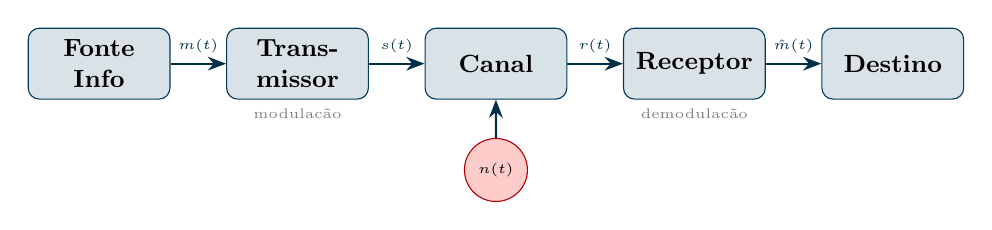
\begin{tikzpicture}[scale=0.9,
  block/.style={rectangle, rounded corners=4pt, draw=unbprimary, fill=unbprimary!15,
                minimum width=1.8cm, minimum height=0.9cm, align=center, font=\small\bfseries},
  noise/.style={circle, draw=red!70!black, fill=red!20, minimum size=0.8cm,
                font=\tiny\bfseries},
  arr/.style={->, thick, >=Stealth, color=unbprimary!80!black}
]
  \node[block] (src)  at (0,0)    {Fonte\\Info};
  \node[block] (tx)   at (2.8,0)  {Trans-\\missor};
  \node[block] (chan) at (5.6,0)  {Canal};
  \node[block] (rx)   at (8.4,0)  {Receptor};
  \node[block] (dst)  at (11.2,0) {Destino};
  \node[noise]  (n)   at (5.6,-1.5) {$n(t)$};
  \draw[arr] (src)  -- node[above, font=\tiny] {$m(t)$} (tx);
  \draw[arr] (tx)   -- node[above, font=\tiny] {$s(t)$} (chan);
  \draw[arr] (chan)  -- node[above, font=\tiny] {$r(t)$} (rx);
  \draw[arr] (rx)   -- node[above, font=\tiny] {$\hat{m}(t)$} (dst);
  \draw[arr] (n)    -- (chan);
  \node[font=\tiny, gray] at (2.8,-0.7) {modulac\~{a}o};
  \node[font=\tiny, gray] at (8.4,-0.7) {demodulac\~{a}o};
\end{tikzpicture}
\end{center}
\vspace{0.1cm}
\begin{columns}
\begin{column}{0.5\textwidth}
  \begin{itemize}
    \item Como \alert{representar} a mensagem como sinal?
    \item Como \alert{transmitir} eficientemente no canal?
  \end{itemize}
\end{column}
\begin{column}{0.5\textwidth}
  \begin{itemize}
    \item Como \alert{combater} o ru\'{\i}do e a distorc\~{a}o?
    \item Qual \'{e} o \alert{limite te\'{o}rico} de desempenho?
  \end{itemize}
\end{column}
\end{columns}
\end{frame}

\begin{frame}{Os tr\^{e}s desafios fundamentais}

Todo sistema de comunicac\~{a}o enfrenta tr\^{e}s quest\~{o}es:

\vspace{0.1cm}

\begin{columns}
\begin{column}{0.32\textwidth}
\begin{center}
\textbf{\textcolor{cBlue}{\Large 1. Espectro}}\\[0.3cm]
\normalsize
Qual largura de banda $B$ o sinal ocupa?\\[0.2cm]
\small R\'{a}dio AM: 10 kHz\\
R\'{a}dio FM: 200 kHz\\
TV: 6 MHz
\end{center}
\end{column}
\begin{column}{0.32\textwidth}
\begin{center}
\textbf{\textcolor{cOrange}{\Large 2. Ru\'{\i}do}}\\[0.3cm]
\normalsize
Como o ru\'{\i}do degrada o sinal recebido?\\[0.2cm]
\small SNR = $P_{\text{sinal}}/P_{\text{ru\'{i}do}}$\\
Quanto maior, melhor!
\end{center}
\end{column}
\begin{column}{0.32\textwidth}
\begin{center}
\textbf{\textcolor{cTeal}{\Large 3. Modulac\~{a}o}}\\[0.3cm]
\normalsize
Como adaptar o sinal ao canal?\\[0.2cm]
\small AM, FM, PM\\
Cada uma com suas vantagens
\end{center}
\end{column}
\end{columns}

\vspace{0.2cm}

\begin{center}
\alert{Esta disciplina ensina a analisar e projetar sistemas que resolvem esses desafios.}
\end{center}
\end{frame}

\begin{frame}{Evoluc\~{a}o dos sistemas de comunicac\~{a}o}
\begin{center}
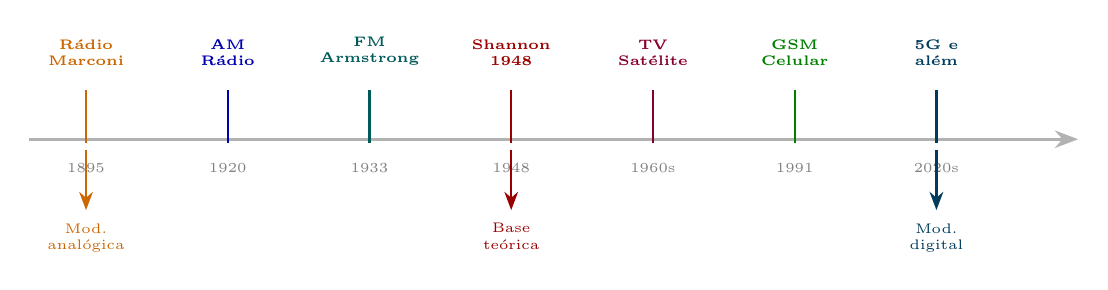
\begin{tikzpicture}[scale=0.9]
  % Linha do tempo principal
  \draw[very thick, -{Stealth}, gray!60] (-0.3, 0) -- (14.5, 0);
  % Ticks e r\'{o}tulos superiores
  \draw[thick, color=cOrange] (0.5,-0.05)--(0.5,0.7);
  \node[above,align=center,font=\tiny\bfseries,color=cOrange] at (0.5,0.9) {R\'{a}dio\\Marconi};
  \node[below,font=\tiny,color=gray] at (0.5,-0.2) {1895};
  \draw[thick, color=cBlue] (2.5,-0.05)--(2.5,0.7);
  \node[above,align=center,font=\tiny\bfseries,color=cBlue] at (2.5,0.9) {AM\\R\'{a}dio};
  \node[below,font=\tiny,color=gray] at (2.5,-0.2) {1920};
  \draw[thick, color=cTeal] (4.5,-0.05)--(4.5,0.7);
  \node[above,align=center,font=\tiny\bfseries,color=cTeal] at (4.5,0.9) {FM\\Armstrong};
  \node[below,font=\tiny,color=gray] at (4.5,-0.2) {1933};
  \draw[thick, color=cRed] (6.5,-0.05)--(6.5,0.7);
  \node[above,align=center,font=\tiny\bfseries,color=cRed] at (6.5,0.9) {Shannon\\1948};
  \node[below,font=\tiny,color=gray] at (6.5,-0.2) {1948};
  \draw[thick, color=cPurple] (8.5,-0.05)--(8.5,0.7);
  \node[above,align=center,font=\tiny\bfseries,color=cPurple] at (8.5,0.9) {TV\\Sat\'{e}lite};
  \node[below,font=\tiny,color=gray] at (8.5,-0.2) {1960s};
  \draw[thick, color=cGreen] (10.5,-0.05)--(10.5,0.7);
  \node[above,align=center,font=\tiny\bfseries,color=cGreen] at (10.5,0.9) {GSM\\Celular};
  \node[below,font=\tiny,color=gray] at (10.5,-0.2) {1991};
  \draw[thick, color=unbprimary] (12.5,-0.05)--(12.5,0.7);
  \node[above,align=center,font=\tiny\bfseries,color=unbprimary] at (12.5,0.9) {5G e\\al\'{e}m};
  \node[below,font=\tiny,color=gray] at (12.5,-0.2) {2020s};
  % Setas e r\'{o}tulos inferiores
  \draw[-{Stealth}, thick, color=cOrange] (0.5,-0.15) -- (0.5,-1.0);
  \node[below,font=\tiny,align=center,color=cOrange] at (0.5,-1.05) {Mod.\\anal\'{o}gica};
  \draw[-{Stealth}, thick, color=cRed] (6.5,-0.15) -- (6.5,-1.0);
  \node[below,font=\tiny,align=center,color=cRed] at (6.5,-1.05) {Base\\te\'{o}rica};
  \draw[-{Stealth}, thick, color=unbprimary] (12.5,-0.15) -- (12.5,-1.0);
  \node[below,font=\tiny,align=center,color=unbprimary] at (12.5,-1.05) {Mod.\\digital};
\end{tikzpicture}
\end{center}
\end{frame}

% ============================================

\begin{frame}{Por que ainda estudar anal\'{o}gico?}
\begin{columns}
\begin{column}{0.48\textwidth}
  \begin{itemize}
    \item Fundamentos de espectro e modulac\~{a}o s\~{a}o \textbf{universais}
    \item R\'{a}dio AM/FM ainda opera em todo o mundo
    \item Entender AM/FM abre a porta para 4G/5G/WiFi
  \end{itemize}
\end{column}
\begin{column}{0.48\textwidth}
  \begin{itemize}
    \item O digital usa portadora, banda, SNR, BW
    \item Fourier, filtros, canal com ru\'{\i}do
    \item \alert{Todos os m\'{o}dulos desta disciplina se conectam!}
  \end{itemize}
\end{column}
\end{columns}
\end{frame}

\begin{frame}{O espectro eletromagn\'{e}tico nas comunicac\~{o}es}
\begin{center}
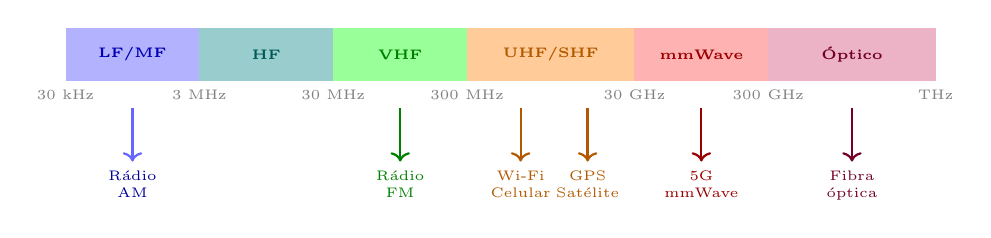
\begin{tikzpicture}[scale=0.85]
  % Barra do espectro
  \fill[blue!30] (0,0) rectangle (2,0.8);
  \fill[teal!40] (2,0) rectangle (4,0.8);
  \fill[green!40] (4,0) rectangle (6,0.8);
  \fill[orange!40] (6,0) rectangle (8.5,0.8);
  \fill[red!30] (8.5,0) rectangle (10.5,0.8);
  \fill[purple!30] (10.5,0) rectangle (13,0.8);
  % Labels de faixa
  \node[font=\tiny\bfseries, text=blue!70!black] at (1,0.4) {LF/MF};
  \node[font=\tiny\bfseries, text=teal!70!black] at (3,0.4) {HF};
  \node[font=\tiny\bfseries, text=green!50!black] at (5,0.4) {VHF};
  \node[font=\tiny\bfseries, text=orange!70!black] at (7.25,0.4) {UHF/SHF};
  \node[font=\tiny\bfseries, text=red!60!black] at (9.5,0.4) {mmWave};
  \node[font=\tiny\bfseries, text=purple!60!black] at (11.75,0.4) {\'{O}ptico};
  % Frequências
  \node[font=\tiny, gray] at (0,-0.2) {30 kHz};
  \node[font=\tiny, gray] at (2,-0.2) {3 MHz};
  \node[font=\tiny, gray] at (4,-0.2) {30 MHz};
  \node[font=\tiny, gray] at (6,-0.2) {300 MHz};
  \node[font=\tiny, gray] at (8.5,-0.2) {30 GHz};
  \node[font=\tiny, gray] at (10.5,-0.2) {300 GHz};
  \node[font=\tiny, gray] at (13,-0.2) {THz};
  % Aplicações (setas para baixo)
  \draw[->, thick, blue!60] (1,-0.4) -- (1,-1.2);
  \node[below, font=\tiny, align=center, text=blue!60!black] at (1,-1.2) {R\'{a}dio\\AM};
  \draw[->, thick, green!50!black] (5,-0.4) -- (5,-1.2);
  \node[below, font=\tiny, align=center, text=green!50!black] at (5,-1.2) {R\'{a}dio\\FM};
  \draw[->, thick, orange!70!black] (6.8,-0.4) -- (6.8,-1.2);
  \node[below, font=\tiny, align=center, text=orange!70!black] at (6.8,-1.2) {Wi-Fi\\Celular};
  \draw[->, thick, orange!70!black] (7.8,-0.4) -- (7.8,-1.2);
  \node[below, font=\tiny, align=center, text=orange!70!black] at (7.8,-1.2) {GPS\\Sat\'{e}lite};
  \draw[->, thick, red!60!black] (9.5,-0.4) -- (9.5,-1.2);
  \node[below, font=\tiny, align=center, text=red!60!black] at (9.5,-1.2) {5G\\mmWave};
  \draw[->, thick, purple!60!black] (11.75,-0.4) -- (11.75,-1.2);
  \node[below, font=\tiny, align=center, text=purple!60!black] at (11.75,-1.2) {Fibra\\\'{o}ptica};
\end{tikzpicture}
\end{center}

\vspace{0.2cm}

\textbf{Nesta disciplina:} aprenderemos a analisar sinais e sistemas em qualquer faixa de frequ\^{e}ncia. Os \textbf{mesmos princ\'{\i}pios} (Fourier, modulac\~{a}o, filtragem) se aplicam do r\'{a}dio AM ao 5G.
\end{frame}

% %%%%%%%%%%%%%%%%%%%%%%%%%%%%%%%%%%%%%%%%%%%%
\section{Roteiro da Disciplina}
% %%%%%%%%%%%%%%%%%%%%%%%%%%%%%%%%%%%%%%%%%%%%

{
\setbeamercolor{background canvas}{bg=unbprimary}
\setbeamercolor{normal text}{fg=white}
\usebeamercolor[fg]{normal text}
\begin{frame}[plain,c]
\begin{center}
{\Huge\textbf{Roteiro da Disciplina}}\\[0.8cm]
{\LARGE O que vamos estudar?}\\[0.5cm]
{\large Tr\^{e}s m\'{o}dulos + laborat\'{o}rio GNU Radio}
\end{center}
\end{frame}
}

\begin{frame}{Vis\~{a}o geral do semestre --- 2026/1}
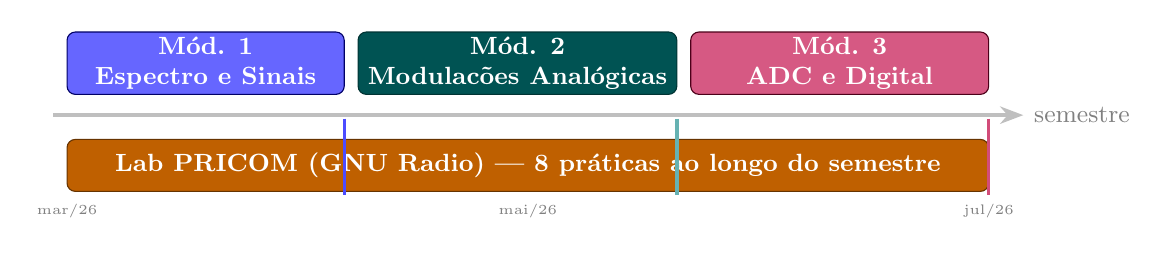
\begin{tikzpicture}[scale=0.88]
  \draw[very thick, -{Stealth}, gray!50] (0, 0) -- (14, 0)
    node[right, font=\small, gray] {semestre};
  \filldraw[fill=blue!60, draw=blue!40!black, rounded corners=3pt]
    (0.2, 0.3) rectangle (4.2, 1.2);
  \node[text=white, font=\small\bfseries, align=center] at (2.2, 0.75)
    {M\'{o}d. 1\\Espectro e Sinais};
  \filldraw[fill=teal!65!black, draw=teal!40!black, rounded corners=3pt]
    (4.4, 0.3) rectangle (9.0, 1.2);
  \node[text=white, font=\small\bfseries, align=center] at (6.7, 0.75)
    {M\'{o}d. 2\\Modulac\~{o}es Anal\'{o}gicas};
  \filldraw[fill=purple!65, draw=purple!40!black, rounded corners=3pt]
    (9.2, 0.3) rectangle (13.5, 1.2);
  \node[text=white, font=\small\bfseries, align=center] at (11.35, 0.75)
    {M\'{o}d. 3\\ADC e Digital};
  \filldraw[fill=orange!75!black, draw=orange!40!black, rounded corners=3pt]
    (0.2, -1.1) rectangle (13.5, -0.35);
  \node[text=white, font=\small\bfseries] at (6.85, -0.73)
    {Lab PRICOM (GNU Radio) --- 8 pr\'{a}ticas ao longo do semestre};
  \draw[very thick, blue!70] (4.2, -0.05) -- (4.2, -1.15);
  \draw[very thick, teal!60] (9.0, -0.05) -- (9.0, -1.15);
  \draw[very thick, purple!70] (13.5, -0.05) -- (13.5, -1.15);
  \node[font=\tiny, gray, below] at (0.2,-1.15)  {mar/26};
  \node[font=\tiny, gray, below] at (6.85,-1.15) {mai/26};
  \node[font=\tiny, gray, below] at (13.5,-1.15) {jul/26};
\end{tikzpicture}
\vspace{0.2cm}
\begin{columns}
\begin{column}{0.33\textwidth}
  \textbf{\textcolor{blue!70!black}{M\'{o}dulo 1:}}\\
  \small Fourier, DEP, DEE, sinais passa-banda
\end{column}
\begin{column}{0.33\textwidth}
  \textbf{\textcolor{teal!60!black}{M\'{o}dulo 2:}}\\
  \small AM, FM, PM, PLL, ru\'{\i}do anal\'{o}gico
\end{column}
\begin{column}{0.33\textwidth}
  \textbf{\textcolor{purple!70}{M\'{o}dulo 3:}}\\
  \small Amostragem, PCM, digital, TEB
\end{column}
\end{columns}
\end{frame}

\begin{frame}{M\'{o}dulo 1 --- Espectro e Sinais}
\begin{columns}
\begin{column}{0.47\textwidth}
  \textbf{Conte\'{u}do:}
  \begin{itemize}
    \item Classificac\~{a}o de sinais (energia, pot\^{e}ncia)
    \item S\'{e}rie de Fourier --- representac\~{a}o espectral
    \item Transformada de Fourier e propriedades
    \item Densidade Espectral de Energia (DEE)
    \item Densidade Espectral de Pot\^{e}ncia (DEP)
    \item Sinais passa-banda e representac\~{a}o complexa
  \end{itemize}
  \vspace{0.1cm}
  \textbf{Livro-texto:}~\cite{lathi2019modern, oppenheim2010signals}
\end{column}
\begin{column}{0.50\textwidth}
  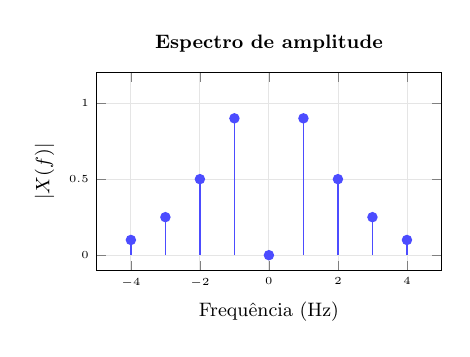
\begin{tikzpicture}[scale=0.78]
  \begin{axis}[
    xlabel={Frequ\^{e}ncia (Hz)}, ylabel={$|X(f)|$},
    xmin=-5, xmax=5, ymin=-0.1, ymax=1.2,
    grid=both, grid style={gray!20},
    width=7.2cm, height=4.8cm,
    tick label style={font=\tiny}, label style={font=\small},
    title style={font=\small\bfseries}, title={Espectro de amplitude},
    ytick={0,0.5,1.0},
  ]
  \addplot[ycomb, thick, color=blue!70, mark=*, mark size=2pt]
    coordinates {(-4,0.1)(-3,0.25)(-2,0.5)(-1,0.9)(0,0.0)
                 (1,0.9)(2,0.5)(3,0.25)(4,0.1)};
  \end{axis}
  \end{tikzpicture}
  \vspace{0.1cm}
  \small Analisador de espectro, FFT no GNU Radio,
  resposta em frequ\^{e}ncia de filtros
\end{column}
\end{columns}
\end{frame}

\begin{frame}{M\'{o}dulo 2 --- Modulac\~{o}es Anal\'{o}gicas}
\begin{columns}
\begin{column}{0.47\textwidth}
  \textbf{Conte\'{u}do:}
  \begin{itemize}
    \item Modulac\~{a}o em Amplitude: DSB-SC, DSB+C, SSB, VSB
    \item Modulac\~{a}o em Frequ\^{e}ncia (FM) e Fase (PM)
    \item \'{I}ndice de modulac\~{a}o, largura de banda (Carson)
    \item Phase-Locked Loop (PLL)
    \item Ru\'{\i}do em sistemas anal\'{o}gicos
    \item RSR nos demoduladores AM e FM
  \end{itemize}
  \vspace{0.1cm}
  \textbf{Livro-texto:}~\cite{lathi2019modern, haykin2009communication}
\end{column}
\begin{column}{0.50\textwidth}
  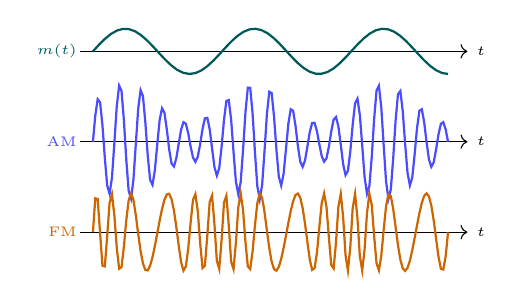
\begin{tikzpicture}[scale=0.82, every node/.style={font=\tiny}]
    \draw[->] (-0.2,2.8) -- (5.8,2.8) node[right]{$t$};
    \draw[thick, teal!70!black, domain=0:5.5, samples=60]
      plot(\x, {2.8 + 0.35*sin(180*\x)});
    \node[left, teal!70!black] at (-0.1, 2.8) {$m(t)$};
    \draw[->] (-0.2,1.4) -- (5.8,1.4) node[right]{$t$};
    \draw[thick, blue!70, domain=0:5.5, samples=150]
      plot(\x, {1.4 + (0.6+0.3*sin(180*\x))*sin(1080*\x)});
    \node[left, blue!70] at (-0.1, 1.4) {AM};
    \draw[->] (-0.2,0.0) -- (5.8,0.0) node[right]{$t$};
    \draw[thick, orange!80!black, domain=0:5.5, samples=150]
      plot(\x, {0.6*sin(1080*\x + 180*sin(180*\x))});
    \node[left, orange!80!black] at (-0.1, 0) {FM};
  \end{tikzpicture}
  \vspace{0.1cm}
  \small R\'{a}dio AM (540--1600 kHz), FM (88--108 MHz)
\end{column}
\end{columns}
\end{frame}

\begin{frame}{M\'{o}dulo 3 --- ADC e Comunicac\~{a}o Digital}
\begin{columns}
\begin{column}{0.47\textwidth}
  \textbf{Conte\'{u}do:}
  \begin{itemize}
    \item Amostragem e teorema de Nyquist-Shannon
    \item Quantizac\~{a}o e codificac\~{a}o PCM
    \item Codificac\~{a}o de linha (NRZ, Manchester, AMI)
    \item Interfer\^{e}ncia Entre S\'{\i}mbolos (ISI)
    \item Taxa de Erro de Bit (TEB) e func\~{a}o $Q$
    \item Noc\~{o}es de protocolos de rede
  \end{itemize}
  \vspace{0.1cm}
  \textbf{Livro-texto:}~\cite{proakis2007fundamentals, lathi2019modern}
\end{column}
\begin{column}{0.50\textwidth}
  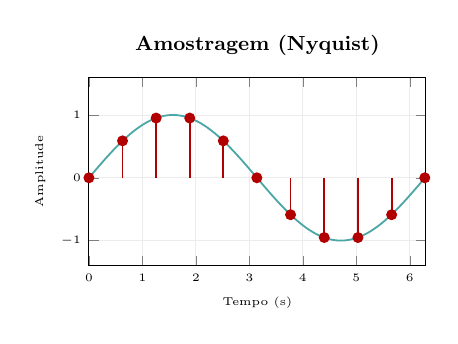
\begin{tikzpicture}[scale=0.82]
  \begin{axis}[
    xlabel={Tempo (s)}, ylabel={Amplitude},
    xmin=0, xmax=6.3, ymin=-1.4, ymax=1.6,
    grid=both, grid style={gray!15},
    width=6.8cm, height=4.5cm,
    tick label style={font=\tiny}, label style={font=\tiny},
    title style={font=\small\bfseries}, title={Amostragem (Nyquist)},
    ytick={-1,0,1}, xtick={0,1,2,3,4,5,6},
  ]
  \addplot[thick, color=teal!70, domain=0:6.28, samples=100]
    { sin(deg(x)) };
  \addplot[ycomb, color=red!70!black, thick, mark=*, mark size=2pt]
    coordinates {(0,0)(0.628,0.588)(1.257,0.951)(1.885,0.951)
                 (2.513,0.588)(3.14,0)(3.77,-0.588)(4.4,-0.951)
                 (5.03,-0.951)(5.66,-0.588)(6.28,0)};
  \end{axis}
  \end{tikzpicture}
  \small CD/MP3, VoIP, WiFi (802.11), 4G LTE, streaming
\end{column}
\end{columns}
\end{frame}

\begin{frame}{Laborat\'{o}rio PRICOM --- GNU Radio}
\begin{columns}
\begin{column}{0.48\textwidth}
  \textbf{8 pr\'{a}ticas experimentais:}
  \begin{enumerate}
    \item An\'{a}lise Espectral (FFT)
    \item Modulac\~{a}o AM DSB-SC
    \item AM Convencional (DSB+C)
    \item Modulac\~{a}o SSB
    \item Modulac\~{a}o FM e Regra de Carson
    \item Phase-Locked Loop (PLL)
    \item Ru\'{\i}do em demoduladores AM vs FM
    \item Amostragem e aliasing
  \end{enumerate}
\end{column}
\begin{column}{0.48\textwidth}
  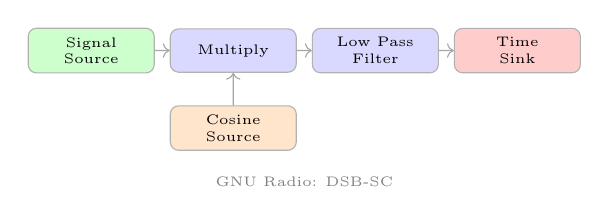
\begin{tikzpicture}[scale=0.82, every node/.style={font=\tiny}]
    \tikzset{
      gnublock/.style={rectangle, rounded corners=3pt, draw=gray!60,
                       fill=blue!15, minimum width=1.6cm, minimum height=0.55cm,
                       align=center, font=\tiny}}
    \node[gnublock, fill=green!20] (src) at (0,2)   {Signal\\Source};
    \node[gnublock] (mul) at (2.2,2)                 {Multiply};
    \node[gnublock, fill=orange!20] (cos) at (2.2,0.8){Cosine\\Source};
    \node[gnublock] (lpf) at (4.4,2)                 {Low Pass\\Filter};
    \node[gnublock, fill=red!20] (snk) at (6.6,2)   {Time\\Sink};
    \draw[->, gray!70] (src) -- (mul);
    \draw[->, gray!70] (cos) -- (mul);
    \draw[->, gray!70] (mul) -- (lpf);
    \draw[->, gray!70] (lpf) -- (snk);
    \node[gray, below, font=\tiny] at (3.3, 0.2) {GNU Radio: DSB-SC};
  \end{tikzpicture}
  \vspace{0.1cm}
  \small Relat\'{o}rio individual por pr\'{a}tica.\\
  $N_L$ = m\'{e}dia dos 8 relat\'{o}rios.
  \vspace{0.2cm}\\
  \alert{Presenças m\'{\i}nimas: 75\% nas pr\'{a}ticas}
\end{column}
\end{columns}
\end{frame}

% %%%%%%%%%%%%%%%%%%%%%%%%%%%%%%%%%%%%%%%%%%%%
\section{Exemplos Motivacionais}
% %%%%%%%%%%%%%%%%%%%%%%%%%%%%%%%%%%%%%%%%%%%%

{
\setbeamercolor{background canvas}{bg=unbprimary}
\setbeamercolor{normal text}{fg=white}
\usebeamercolor[fg]{normal text}
\begin{frame}[plain,c]
\begin{center}
{\Huge\textbf{Exemplos Motivacionais}}\\[0.8cm]
{\LARGE Como os conceitos aparecem na pr\'{a}tica?}\\[0.5cm]
{\large AM, FM, celular, GPS, satélite \ldots}
\end{center}
\end{frame}
}

\begin{frame}{R\'{a}dio AM e FM --- o cl\'{a}ssico que ainda funciona}
\begin{columns}
\begin{column}{0.50\textwidth}
  \textbf{R\'{a}dio AM (540--1600 kHz):}
  \begin{itemize}
    \item $s(t) = A_c[1 + \mu m(t)]\cos(2\pi f_c t)$
    \item Demodulac\~{a}o simples: detector de envolt\'{o}ria
    \item Alcance longo; \alert{problem:} suscet\'{\i}vel ao ru\'{\i}do
  \end{itemize}
  \vspace{0.1cm}
  \textbf{R\'{a}dio FM (88--108 MHz):}
  \begin{itemize}
    \item Frequ\^{e}ncia varia: $f_i(t) = f_c + k_f m(t)$
    \item Carson: $B \approx 2(\Delta f + f_m)$
    \item \alert{Vantagem:} alta imunidade ao ru\'{\i}do
    \item Melhor qualidade de \'{a}udio (est\'{e}reo)
  \end{itemize}
\end{column}
\begin{column}{0.47\textwidth}
  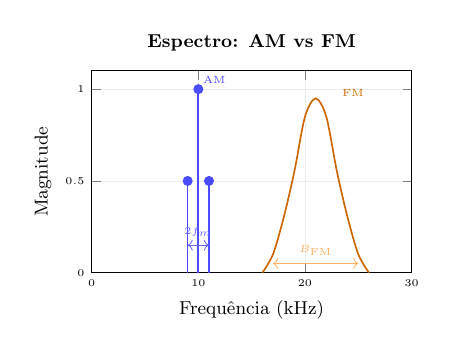
\begin{tikzpicture}[scale=0.75]
  \begin{axis}[
    xlabel={Frequ\^{e}ncia (kHz)}, ylabel={Magnitude},
    xmin=0, xmax=30, ymin=0, ymax=1.1,
    grid=both, grid style={gray!15},
    width=7cm, height=5cm,
    tick label style={font=\tiny}, label style={font=\small},
    title style={font=\small\bfseries}, title={Espectro: AM vs FM},
  ]
  \addplot[ycomb, thick, color=blue!70, mark=*, mark size=2pt]
    coordinates {(9,0.5)(10,1.0)(11,0.5)};
  \node[font=\tiny, text=blue!70] at (axis cs:11.5,1.05) {AM};
  \addplot[thick, color=orange!80!black, smooth]
    coordinates {(16,0)(17,0.1)(18,0.3)(19,0.55)(20,0.85)(21,0.95)
                 (22,0.85)(23,0.55)(24,0.3)(25,0.1)(26,0)};
  \node[font=\tiny, text=orange!80!black] at (axis cs:24.5,0.98) {FM};
  \draw[<->, thin, color=blue!60] (axis cs:9,0.15) -- (axis cs:11,0.15);
  \node[font=\tiny, text=blue!60] at (axis cs:10,0.22) {$2f_m$};
  \draw[<->, thin, color=orange!60] (axis cs:17,0.05) -- (axis cs:25,0.05);
  \node[font=\tiny, text=orange!60] at (axis cs:21,0.12) {$B_{\rm FM}$};
  \end{axis}
  \end{tikzpicture}
\end{column}
\end{columns}
\end{frame}

\begin{frame}{Largura de banda: o recurso mais precioso}
\begin{columns}
\begin{column}{0.55\textwidth}
  \textbf{Cada sistema ocupa uma ``fatia'' do espectro:}

  \vspace{0.2cm}

  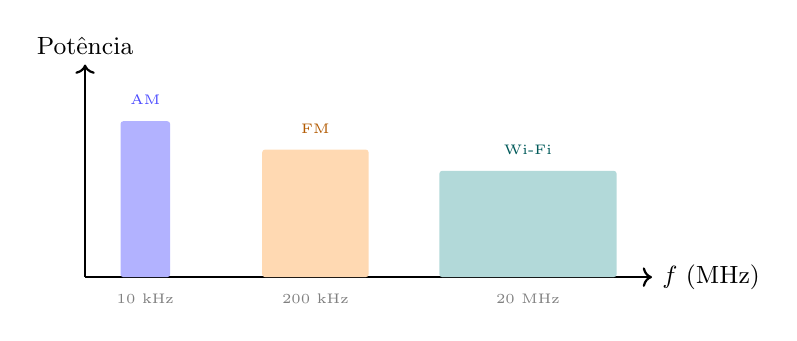
\begin{tikzpicture}[scale=0.9]
    \draw[->, thick] (0,0) -- (8,0) node[right, font=\small] {$f$ (MHz)};
    \draw[->, thick] (0,0) -- (0,3) node[above, font=\small] {Pot\^{e}ncia};
    % AM
    \fill[blue!30, rounded corners=1pt] (0.5,0) rectangle (1.2,2.2);
    \node[font=\tiny, text=blue!70] at (0.85,2.5) {AM};
    \node[font=\tiny, gray] at (0.85,-0.3) {10 kHz};
    % FM
    \fill[orange!30, rounded corners=1pt] (2.5,0) rectangle (4.0,1.8);
    \node[font=\tiny, text=orange!70!black] at (3.25,2.1) {FM};
    \node[font=\tiny, gray] at (3.25,-0.3) {200 kHz};
    % WiFi
    \fill[teal!30, rounded corners=1pt] (5.0,0) rectangle (7.5,1.5);
    \node[font=\tiny, text=teal!70!black] at (6.25,1.8) {Wi-Fi};
    \node[font=\tiny, gray] at (6.25,-0.3) {20 MHz};
  \end{tikzpicture}
\end{column}
\begin{column}{0.42\textwidth}
  \textbf{Por que importa?}
  \begin{itemize}
    \item Espectro \'{e} \textbf{finito} e regulado (Anatel)
    \item Mais banda $\rightarrow$ mais informac\~{a}o
    \item AM: 10 kHz (voz)
    \item FM: 200 kHz (\'{a}udio hi-fi)
    \item Wi-Fi: 20 MHz (dados)
    \item 5G: at\'{e} 400 MHz!
  \end{itemize}

  \vspace{0.2cm}

  \alert{Entender espectro \'{e} essencial!}
\end{column}
\end{columns}
\end{frame}

\begin{frame}{Do r\'{a}dio ao celular --- mesmos fundamentos}

\begin{center}
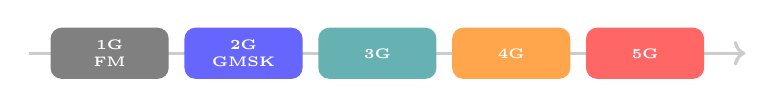
\begin{tikzpicture}[scale=0.85]
    \draw[->, very thick, gray!40] (-1.2,0) -- (9.5,0);
    \node[rounded corners, fill=gray, text=white, minimum width=1.5cm,
          minimum height=0.65cm, align=center, font=\tiny\bfseries] at (0,0) {1G\\FM};
    \node[rounded corners, fill=blue!60, text=white, minimum width=1.5cm,
          minimum height=0.65cm, align=center, font=\tiny\bfseries] at (2,0) {2G\\GMSK};
    \node[rounded corners, fill=teal!60, text=white, minimum width=1.5cm,
          minimum height=0.65cm, align=center, font=\tiny\bfseries] at (4,0) {3G};
    \node[rounded corners, fill=orange!70, text=white, minimum width=1.5cm,
          minimum height=0.65cm, align=center, font=\tiny\bfseries] at (6,0) {4G};
    \node[rounded corners, fill=red!60, text=white, minimum width=1.5cm,
          minimum height=0.65cm, align=center, font=\tiny\bfseries] at (8,0) {5G};
\end{tikzpicture}
\end{center}

\textbf{O que \'{e} comum a todas as gerac\~{o}es?}
\begin{columns}
\begin{column}{0.48\textwidth}
  \begin{itemize}
    \item Portadora de r\'{a}dio-frequ\^{e}ncia
    \item Modulac\~{a}o do sinal na portadora
  \end{itemize}
\end{column}
\begin{column}{0.48\textwidth}
  \begin{itemize}
    \item An\'{a}lise de espectro e largura de banda
    \item Combate ao ru\'{\i}do e distorc\~{a}o do canal
  \end{itemize}
\end{column}
\end{columns}

\end{frame}

% ============================================

\begin{frame}{O 1G era FM anal\'{o}gica pura!}

O celular original (\textbf{AMPS}, 1983) usava exatamente a modulac\~{a}o FM que estudaremos no M\'{o}dulo 2.

\vspace{0.3cm}

\textbf{Conceitos desta disciplina aplicados a celular:}
\begin{itemize}
  \item \textbf{M\'{o}d. 1:} Espectro e filtros --- como o sinal ocupa a banda
  \item \textbf{M\'{o}d. 2:} AM, FM --- a base de toda comunicac\~{a}o sem fio
  \item \textbf{M\'{o}d. 3:} Amostragem e digitalizac\~{a}o --- a transic\~{a}o para 2G em diante
\end{itemize}

\vspace{0.3cm}

\alert{Sem entender AM/FM, n\~{a}o se entende 4G/5G!}

\end{frame}

% %%%%%%%%%%%%%%%%%%%%%%%%%%%%%%%%%%%%%%%%%%%%
\section{Avalia\c{c}\~{a}o}
% %%%%%%%%%%%%%%%%%%%%%%%%%%%%%%%%%%%%%%%%%%%%

{
\setbeamercolor{background canvas}{bg=unbprimary}
\setbeamercolor{normal text}{fg=white}
\usebeamercolor[fg]{normal text}
\begin{frame}[plain,c]
\begin{center}
{\Huge\textbf{Avaliac\~{a}o}}\\[0.8cm]
{\LARGE Como a disciplina \'{e} avaliada?}\\[0.5cm]
{\large Teoria (75\%) + Laborat\'{o}rio (25\%)}
\end{center}
\end{frame}
}

\begin{frame}{Componentes da avaliac\~{a}o}
\begin{columns}
\begin{column}{0.52\textwidth}
  \begin{block}{Nota Te\'{o}rica ($N_T$)}
  \vspace{-4pt}
  \[\textstyle
    N_T = \frac{P_1 + P_2 + 2P_3}{4}
  \]
  \vspace{-6pt}
  \begin{itemize}\setlength{\itemsep}{0pt}
    \item $P_1$: ao final do M\'{o}dulo 1
    \item $P_2$: ao final do M\'{o}dulo 2
    \item $P_3$: M\'{o}dulo 3 (peso 2) --- \alert{obrigat\'{o}ria}
  \end{itemize}
  \vspace{-2pt}
  \end{block}
  \vspace{0.1cm}
  \begin{block}{Nota de Laborat\'{o}rio ($N_L$)}
  \vspace{-4pt}
  \[\textstyle
    N_L = \frac{\sum_{k=1}^{8} \text{Rel}_k}{8}
  \]
  \vspace{-6pt}
  \footnotesize Relat\'{o}rio individual por pr\'{a}tica (8 no total)
  \vspace{-2pt}
  \end{block}
\end{column}
\begin{column}{0.45\textwidth}
  \begin{block}{Nota Final ($N_F$)}
  \[
    N_F = 0{,}75\,N_T + 0{,}25\,N_L
  \]
  \end{block}
  \vspace{0.1cm}
  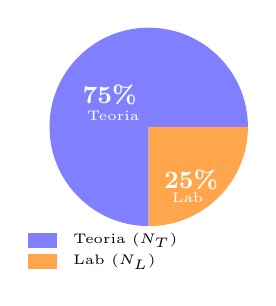
\begin{tikzpicture}[scale=0.9]
    \fill[blue!50] (0,0) -- (1.4,0) arc (0:270:1.4) -- cycle;
    \fill[orange!70] (0,0) -- (0,-1.4) arc (270:360:1.4) -- cycle;
    \node[font=\small\bfseries, text=white] at (-0.55, 0.45) {75\%};
    \node[font=\tiny, text=white] at (-0.5, 0.15) {Teoria};
    \node[font=\small\bfseries, text=white] at (0.6,-0.75) {25\%};
    \node[font=\tiny, text=white] at (0.55,-1.0) {Lab};
    \filldraw[blue!50] (-1.7,-1.7) rectangle (-1.3,-1.5);
    \node[right, font=\tiny] at (-1.2,-1.6) {Teoria ($N_T$)};
    \filldraw[orange!70] (-1.7,-2.0) rectangle (-1.3,-1.8);
    \node[right, font=\tiny] at (-1.2,-1.9) {Lab ($N_L$)};
  \end{tikzpicture}
\end{column}
\end{columns}
\end{frame}

\begin{frame}{Condic\~{o}es de aprovac\~{a}o e frequ\^{e}ncia}
\begin{columns}
\begin{column}{0.50\textwidth}
  \begin{alertblock}{Condic\~{o}es obrigat\'{o}rias}
  \begin{enumerate}
    \item $N_T \geq 5{,}0$ \textbf{e} $N_L \geq 5{,}0$
    \item $N_F \geq 5{,}0$
    \item Frequ\^{e}ncia $\geq 75\%$ nas aulas te\'{o}ricas
    \item Presenc\~{a} $\geq 75\%$ nas pr\'{a}ticas de lab
    \item \alert{Obrigat\'{o}rio realizar P3}
  \end{enumerate}
  \end{alertblock}
  \vspace{0.2cm}
 %\begin{exampleblock}{Dica}
 %Alunos que fazem \textbf{todas as pr\'{a}ticas} com boa qualidade
 %garantem $N_L$ alta e aliviam a press\~{a}o nas provas!
 %\end{exampleblock}
\end{column}
\begin{column}{0.47\textwidth}
  \textbf{Cronograma 2026/1:}
  \vspace{0.1cm}
  \begin{tabular}{ll}
    \hline
    \textbf{Evento} & \textbf{Data} \\
    \hline
    In\'{\i}cio das aulas  & 16/03/2026 \\
    Prova 1 (P1)       & Semana de 20/04 \\
    Prova 2 (P2)       & Semana de 08/06 \\
    Prova 3 (P3)       & Semana de 13/07 \\
    Fim do semestre    & 18/07/2026 \\
    \hline
  \end{tabular}
  \vspace{0.2cm}\\
  \textbf{Contato:}\\
  \href{mailto:\autorEmail}{\autorEmail}\\
  Microsoft Teams / SIGAA
\end{column}
\end{columns}
\end{frame}

% %%%%%%%%%%%%%%%%%%%%%%%%%%%%%%%%%%%%%%%%%%%%
\section{Instalac\~{a}o do GNU Radio}
% %%%%%%%%%%%%%%%%%%%%%%%%%%%%%%%%%%%%%%%%%%%%

{
\setbeamercolor{background canvas}{bg=unbprimary}
\setbeamercolor{normal text}{fg=white}
\usebeamercolor[fg]{normal text}
\begin{frame}[plain,c]
\begin{center}
{\Huge\textbf{Laborat\'{o}rio PRICOM}}\\[0.8cm]
{\LARGE Instalac\~{a}o do GNU Radio}\\[0.5cm]
{\large Radioconda --- distribuic\~{a}o pronta para SDR}
\end{center}
\end{frame}
}

\begin{frame}{Por que o Radioconda?}
\begin{columns}
\begin{column}{0.55\textwidth}
  \textbf{O que \'{e} o Radioconda?}
  \begin{itemize}
    \item Distribuic\~{a}o baseada em Conda com:\\
      GNU Radio + bibliotecas SDR prontas
    \item Evita conflitos de depend\^{e}ncias do sistema
    \item Mesma experi\^{e}ncia no Windows, Linux e macOS
    \item Inclui: GNU Radio, gr-osmosdr, SoapySDR, UHD\ldots
  \end{itemize}
  \vspace{0.1cm}
  \textbf{Reposit\'{o}rio oficial:}\\
  {\footnotesize\url{https://github.com/radioconda/radioconda-installer}}
\end{column}
\begin{column}{0.42\textwidth}
  \textbf{Vantagens:}
  \begin{itemize}
    \item Instalac\~{a}o simples e r\'{a}pida
    \item Multiplataforma
    \item Todas as depend\^{e}ncias inclusas
  \end{itemize}
\end{column}
\end{columns}
\end{frame}

\begin{frame}{Radioconda: componentes}
\begin{columns}
\begin{column}{0.55\textwidth}
  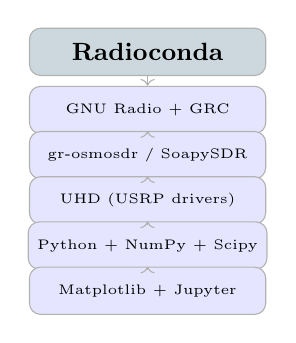
\begin{tikzpicture}[scale=0.82, every node/.style={font=\tiny}]
    \tikzset{pkg/.style={rectangle, rounded corners=4pt, draw=gray!60,
                         fill=blue!10, minimum width=3.0cm, minimum height=0.6cm,
                         align=center, font=\tiny}}
    \node[pkg, fill=unbprimary!20, font=\small\bfseries] (rc) at (0,3.5) {Radioconda};
    \node[pkg] (gnr) at (0,2.6) {GNU Radio + GRC};
    \node[pkg] (osr) at (0,1.9) {gr-osmosdr / SoapySDR};
    \node[pkg] (uhd) at (0,1.2) {UHD (USRP drivers)};
    \node[pkg] (py)  at (0,0.5) {Python + NumPy + Scipy};
    \node[pkg] (mpl) at (0,-0.2) {Matplotlib + Jupyter};
    \foreach \a/\b in {rc/gnr, gnr/osr, osr/uhd, uhd/py, py/mpl}
      \draw[->, gray!60] (\a) -- (\b);
  \end{tikzpicture}
\end{column}
\begin{column}{0.42\textwidth}
  \begin{alertblock}{Aten\c{c}\~{a}o --- laborat\'{o}rio presencial}
  Se os computadores \textbf{n\~{a}o tiverem} o GNU Radio instalado,
  baixe o instalador Windows \textbf{antes da aula} e leve num pen-drive!
  \end{alertblock}
\end{column}
\end{columns}
\end{frame}

\begin{frame}{Download do Radioconda --- Linux/macOS}
\begin{columns}
\begin{column}{0.50\textwidth}
  \textbf{Linux / macOS:}
  \begin{enumerate}
    \item Acesse o reposit\'{o}rio oficial:\\
      {\footnotesize\url{https://github.com/radioconda/radioconda-installer}}
    \item Baixe o instalador para seu sistema
    \item Siga as instru\c{c}\~{o}es do README
  \end{enumerate}
\end{column}
\begin{column}{0.47\textwidth}
  \begin{exampleblock}{Dica: baixe antes da aula}
  O arquivo de instalac\~{a}o tem $\sim$1--2 GB.\\
  Baixe em casa e leve num pen-drive para n\~{a}o depender
  da internet do laborat\'{o}rio.
  \end{exampleblock}
\end{column}
\end{columns}
\end{frame}

\begin{frame}{Download do Radioconda --- Windows}
\begin{columns}
\begin{column}{0.50\textwidth}
  \textbf{Windows (para o laborat\'{o}rio):}
  \begin{enumerate}
    \item Baixe o instalador \texttt{.exe} diretamente pelo link:\\
      {\tiny\url{https://glare-sable.vercel.app/radioconda/radioconda-installer/radioconda-.*-Windows-x86_64.exe}}
    \item Execute com permiss\~{a}o de administrador
    \item Siga o assistente de instalac\~{a}o
    \item Aguarde a instalac\~{a}o ($\sim$10--20 min)
  \end{enumerate}
\end{column}
\begin{column}{0.47\textwidth}
  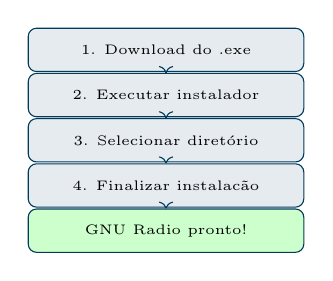
\begin{tikzpicture}[scale=0.82, every node/.style={font=\tiny}]
    \tikzset{flowstep/.style={rectangle, rounded corners=3pt, draw=unbprimary,
                          fill=unbprimary!10, minimum width=3.5cm,
                          minimum height=0.55cm, align=center, font=\tiny}}
    \node[flowstep] (d) at (0, 2.4) {1. Download do .exe};
    \node[flowstep] (i) at (0, 1.7) {2. Executar instalador};
    \node[flowstep] (p) at (0, 1.0) {3. Selecionar diret\'{o}rio};
    \node[flowstep] (f) at (0, 0.3) {4. Finalizar instalac\~{a}o};
    \node[flowstep, fill=green!20] (ok) at (0,-0.4) {GNU Radio pronto!};
    \foreach \a/\b in {d/i, i/p, p/f, f/ok}
      \draw[->, unbprimary] (\a) -- (\b);
  \end{tikzpicture}
\end{column}
\end{columns}
\end{frame}

\begin{frame}{Usando o Radioconda no Windows --- passo a passo}
\begin{columns}
\begin{column}{0.50\textwidth}
  \textbf{Ap\'{o}s a instalac\~{a}o:}
  \begin{enumerate}
    \item Abra o \textbf{Menu Iniciar}
    \item Procure a pasta \textbf{``radioconda''}
    \item Clique em \textbf{``radioconda Prompt''}
    \item No terminal aberto, execute:
  \end{enumerate}
  \vspace{0.1cm}
  \begin{block}{Comandos \'{u}teis no radioconda Prompt}
  \begin{itemize}
    \item Abrir GNU Radio Companion:\\
      \texttt{gnuradio-companion}
    \item Atualizar pacotes:\\
      \texttt{mamba update -{}-all}
    \item Instalar pacote adicional:\\
      \texttt{mamba install <pacote>}
  \end{itemize}
  \end{block}
\end{column}
\begin{column}{0.47\textwidth}
  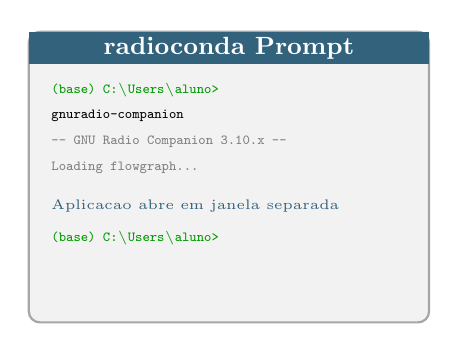
\begin{tikzpicture}[scale=0.82, every node/.style={font=\tiny}]
    % Janela de terminal estilizada
    \draw[rounded corners=4pt, thick, gray!70, fill=gray!10]
      (0,0) rectangle (6.2, 4.5);
    \fill[unbprimary!80] (0,4.0) rectangle (6.2,4.5);
    \node[text=white, font=\small\bfseries] at (3.1,4.25) {radioconda Prompt};
    \node[right, font=\ttfamily\tiny, text=green!60!black] at (0.2,3.6)
      {(base) C:\textbackslash{}Users\textbackslash{}aluno>};
    \node[right, font=\ttfamily\tiny] at (0.2,3.2)
      {gnuradio-companion};
    \node[right, font=\ttfamily\tiny, text=gray] at (0.2,2.8)
      {-- GNU Radio Companion 3.10.x --};
    \node[right, font=\ttfamily\tiny, text=gray] at (0.2,2.4)
      {Loading flowgraph...};
    \node[right, font=\tiny, text=unbprimary!80] at (0.2,1.8)
      {Aplicacao abre em janela separada};
    \node[right, font=\ttfamily\tiny, text=green!60!black] at (0.2,1.3)
      {(base) C:\textbackslash{}Users\textbackslash{}aluno>};
  \end{tikzpicture}
  \vspace{0.2cm}
  \small O GRC abre em janela separada.\\
  Atalhos na pasta \textbf{radioconda} do\\
  menu iniciar tamb\'{e}m funcionam.
\end{column}
\end{columns}
\end{frame}

\begin{frame}{Verificando a instalac\~{a}o}
\begin{columns}
\begin{column}{0.50\textwidth}
  \textbf{Teste r\'{a}pido no radioconda Prompt:}
  \vspace{0.1cm}
  \begin{block}{Verificar vers\~{a}o do GNU Radio}
  {\small\texttt{python -c "import gnuradio;}\\\texttt{print(gnuradio.version())"}}
  \end{block}
  \vspace{0.1cm}
  \begin{block}{Verificar NumPy e SciPy}
  {\small\texttt{python -c "import numpy, scipy;}\\\texttt{print('OK')"}}
  \end{block}
\end{column}
\begin{column}{0.47\textwidth}
  \begin{exampleblock}{Sucesso!}
  Se aparecer a vers\~{a}o e ``OK'':\\
  Tudo instalado corretamente.\\
  Voc\^{e} est\'{a} pronto para as pr\'{a}ticas!
  \end{exampleblock}
\end{column}
\end{columns}
\end{frame}

\begin{frame}{Problemas comuns na instalac\~{a}o}
\begin{columns}
\begin{column}{0.50\textwidth}
  \textbf{Problemas comuns:}
  \begin{itemize}
    \item \textbf{``command not found''}:\\
      Abrir pelo menu iniciar, n\~{a}o pelo CMD padr\~{a}o
    \item \textbf{Tela preta do GRC}:\\
      Reinstalar drivers de v\'{\i}deo ou usar\\
      \texttt{-{}-no-opengl}
    \item \textbf{Erro de permiss\~{a}o}:\\
      Executar o instalador como Administrador
    \item \textbf{Espac\~{a}o insuficiente}:\\
      A instalac\~{a}o requer $\geq 5$ GB livres
  \end{itemize}
\end{column}
\begin{column}{0.47\textwidth}
  \begin{alertblock}{Suporte}
  Em caso de d\'{u}vida, consulte o professor
  antes da aula de laborat\'{o}rio.
  \end{alertblock}
\end{column}
\end{columns}
\end{frame}

% %%%%%%%%%%%%%%%%%%%%%%%%%%%%%%%%%%%%%%%%%%%%
\section{Pr\'{e}-requisitos e Ferramentas}
% %%%%%%%%%%%%%%%%%%%%%%%%%%%%%%%%%%%%%%%%%%%%

{
\setbeamercolor{background canvas}{bg=unbprimary}
\setbeamercolor{normal text}{fg=white}
\usebeamercolor[fg]{normal text}
\begin{frame}[plain,c]
\begin{center}
{\Huge\textbf{Pr\'{e}-requisitos e Ferramentas}}\\[0.8cm]
{\LARGE O que voc\^{e} j\'{a} deve saber}
\end{center}
\end{frame}
}

\begin{frame}{Pr\'{e}-requisitos e por que esta disciplina importa}
\begin{columns}
\begin{column}{0.48\textwidth}
  \begin{block}{Pr\'{e}-requisitos}
  \textbf{FGA0102 --- Sinais e Sistemas:}
  \begin{itemize}
    \item Transformada de Fourier (revis\~{a}o)
    \item Sistemas LTI, resposta em frequ\^{e}ncia
    \item Convoluc\~{a}o e filtragem
  \end{itemize}
  \vspace{0.2cm}
  \textbf{FGA0067 --- Circuitos I:}
  \begin{itemize}
    \item An\'{a}lise no dom\'{\i}nio da frequ\^{e}ncia
    \item Osciladores e filtros b\'{a}sicos
  \end{itemize}
  \end{block}
  \vspace{0.1cm}
  %\alert{N\~{a}o se preocupe se n\~{a}o recorda tudo ---
  %revisaremos os fundamentos no in\'{\i}cio do M\'{o}dulo 1!}
\end{column}
\begin{column}{0.48\textwidth}
  \textbf{Portas que a PRICOM abre:}
  \begin{itemize}
    \item Comunicac\~{o}es Digitais Avanc\~{a}das
    \item Redes sem Fio (Wi-Fi, 5G, LoRa)
    \item Processamento de Sinais
    \item SDR / HackRF / USRP
    \item IoT, Sistemas Embarcados
  \end{itemize}
  \vspace{0.1cm}
  \textbf{Na ind\'{u}stria, voc\^{e} vai usar:}
  \begin{itemize}
    \item An\'{a}lise de espectro em telemetria
    \item Dimensionamento de enlaces de rede
    \item C\'{a}lculo de SNR e taxa de erro
    \item Protocolos: 4G, 5G, LoRa, BLE
  \end{itemize}
\end{column}
\end{columns}
\end{frame}

% ============================================
% ENCERRAMENTO
% ============================================
\begin{frame}{Bem-vindos \`{a} disciplina!}
\begin{center}
\Large \textbf{Princ\'{\i}pios de Comunicac\~{a}o para Engenharia}\\
\large FGA0092 --- 2026/1
\vspace{0.8cm}

\normalsize
\textbf{Prof.} \autorNome\\
\href{mailto:\autorEmail}{\autorEmail}
\vspace{0.2cm}

\textbf{\laboratorioFinal}\\
\universidadeFinal
\vspace{0.7cm}

\begin{columns}
\begin{column}{0.33\textwidth}
\centering
\textbf{D\'{u}vidas:}\\
\small E-mail / Teams
\end{column}
\begin{column}{0.33\textwidth}
\centering
\textbf{Material:}\\
\small SIGAA
\end{column}
\begin{column}{0.33\textwidth}
\centering
\textbf{In\'{\i}cio:}\\
\small 16/03/2026
\end{column}
\end{columns}

\vspace{0.7cm}
\large \alert{Vamos come\c{c}ar?}
\end{center}
\end{frame}

% ============================================
% REFERÊNCIAS
% ============================================
\begin{frame}[allowframebreaks]{Refer\^{e}ncias}
\nocite{*}
\bibliographystyle{ieeetr}
\bibliography{references}
\end{frame}

\end{document}
